\documentclass{beamer}

\usepackage{pgfpages}
% Note rendering settings
% \setbeameroption{hide notes} % Default
% \setbeameroption{show notes}
% \setbeameroption{show only notes}
% \setbeameroption{show notes on second screen}

% Maths
\usepackage{mathabx}
\usepackage{mathtools}

% Support for sane handling of values with SI units
\usepackage{siunitx}

% Algorithms using algorithmicx package (with its algpseudocode command set)
\usepackage{algpseudocode}

% Code listings
\usepackage{listings}
\usepackage{lstautogobble}
\lstset{
		basicstyle=\small,
		breaklines=true,
		autogobble=true,
		postbreak=\mbox{$\drsh$},
}

% Date management
\usepackage{datetime2}
\DTMsavedate{presentation}{2022-06-02}

% BibLaTeX
\usepackage[
  style=alphabetic,
  backend=biber, % Default backend, just listed for completness
  sorting=ynt % Sort by year, name, title
]{biblatex}
\addbibresource{references.bib}
\nocite{*}

% A more modern (and less beamer-y) theme
\usetheme{metropolis}

% \metroset{sectionpage=simple}
% Optional light gray fill behind block environments such as \theorem
% \metroset{block=fill}

\title{SuRF: Succinct Range Filters}
\subtitle{Probabilistic point- and range-membership checks}
\author{Michael Senn}
\institute{Faculty of Science, University of Bern}
\date{\DTMusedate{presentation}}

\begin{document}

\maketitle

% Only show sections
% \setcounter{tocdepth}{1}
\begin{frame}{Outline}
		\tableofcontents
\end{frame}

% • A motivation (what problem was the data structure designed to solve?)
% • General layout of the data structure
% • Lookup
% • Insertion/Loading
% • Performance relative to alternative structures
% • Critique

\section{Motivation}

\begin{frame}{Goal}
		\begin{itemize}
				\item \textbf{Goal}: Probabilistic point- and range-membership queries
						\begin{itemize}
								\item Let $X$ be set of keys (e.g. arbitrary byte sequences)
								\item $\operatorname{Point}(x) \coloneqq x \overset{?}{\in} X$
								\item $\operatorname{Range}(a, b) \coloneqq x \overset{?}{\in} X : a \leq x \leq b$
								\item $\operatorname{Count}(a, b) \coloneqq |\{x \in X : a \leq x \leq b\}|$
						\end{itemize}
				\item Potential for false-positives (respectively
						over-counting), but no false negatives (respectively
						under-counting)
				\item Compare with Bloom filter: Only point-membership
				\item Optional: Associate fixed-size value with each key
				\item Use case of authors: Replacement for bloom filter in
						RocksDB, an LSM-based KV store.
		\end{itemize}
\end{frame}

\begin{frame}{Non-Goal}
		\begin{itemize}
				\item No addition of keys, data structure populated with keys
						only during initializaiton
						\begin{itemize}
								\item Can be done, but not described in paper
						\end{itemize}
				\item No updates or deletion of keys
				\item Fully in-memory
				\item Less tight / rigorous bounds on false-positive error rate
		\end{itemize}
\end{frame}

\section{Data structure layout}

\begin{frame}{How to efficiently encode a trie?}
		\begin{columns}
				\column{0.3\textwidth}
				\begin{figure}
						\centering
						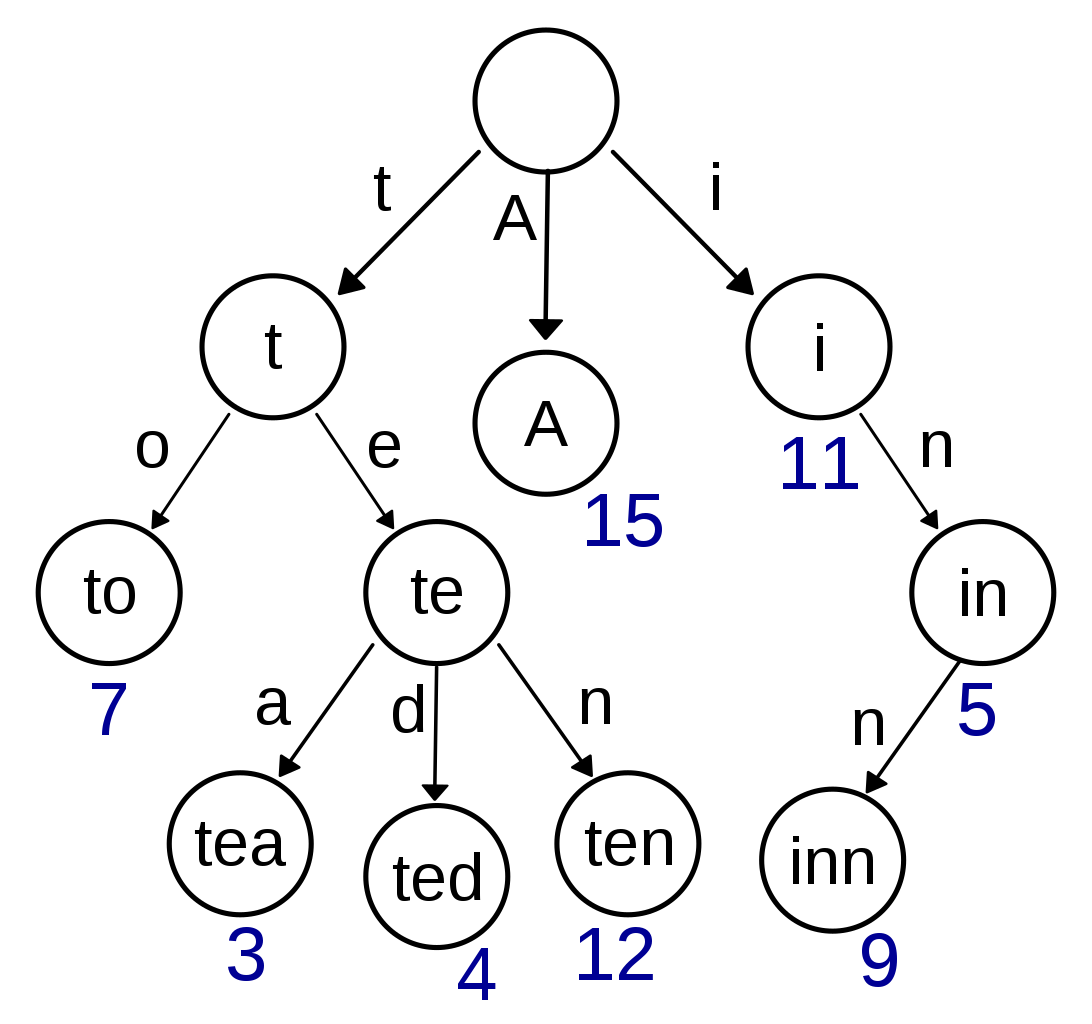
\includegraphics[width=\textwidth]{resources/trie.png}
						\caption{Wikimedia \autocite{booyabazookaTrieExampleSvg}}
				\end{figure}
				\column{0.7\textwidth}
				\begin{itemize}
						\item Assume trie of bytes, 64bit architecture
						\item Naive approach: For each edge, store its value and
								pointers to child node
						\item Then $k \cdot (8 + 64)$ bit for $k$-child node
						\item Hugely inefficient. Encoding \qty{1}{\byte} costs
								\qty{9}{\byte}!
				\end{itemize}
		\end{columns}
\end{frame}

\begin{frame}{LOUDS: Efficient encoding of ordinal trees}
		\begin{columns}
				\column{0.4\textwidth}
				\begin{figure}
						\centering
						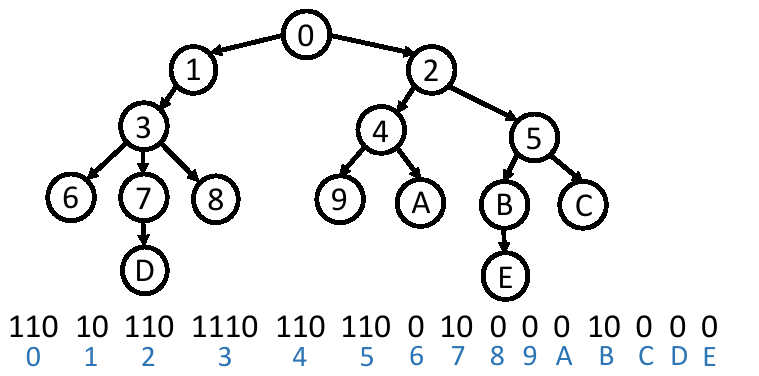
\includegraphics[width=\textwidth]{resources/trie_louds.png}
						\caption{\autocite{zhangSuRFPracticalRange2018}}
				\end{figure}
				\column{0.6\textwidth}
				\begin{itemize}
						\item LOUDS: Level-order unary degree sequence \autocite{jacobsonSpaceefficientStaticTrees1989}
						\item Node with $n$ children: $n$ $1$s, followed by one $0$
						\item Can be navigated with $\operatorname{rank}$ and
								$\operatorname{select}$ operations
						\item Which can be made constant-time by utilizing LUTs
				\end{itemize}
		\end{columns}
\end{frame}

\begin{frame}{FST: Fast succinct tries}
		\begin{itemize}
				\item Observation
						\begin{itemize}
								\item Upper levels of tries have many edges, lower levels have few
								\item Yet most accesses to nodes of upper level
						\end{itemize}
				\item LOUDS variants to accomodate this
				\item LOUDS-DENSE for upper levels: Optimized for fast lookup
				\item LOUDS-SPARSE for lower levels: Optimized for compact storage
		\end{itemize}
\end{frame}

\begin{frame}{LOUDS-DENSE}
		\begin{columns}
				\column{0.4\textwidth}
				\begin{figure}
						\centering
						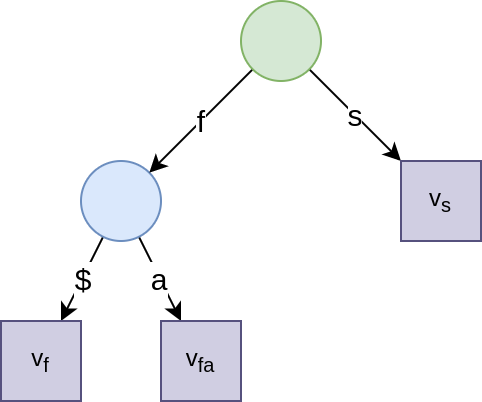
\includegraphics[width=\textwidth]{resources/louds_trie}
						\caption{Example FST}
				\end{figure}
				\column{0.6\textwidth}
				\begin{figure}
						\centering
						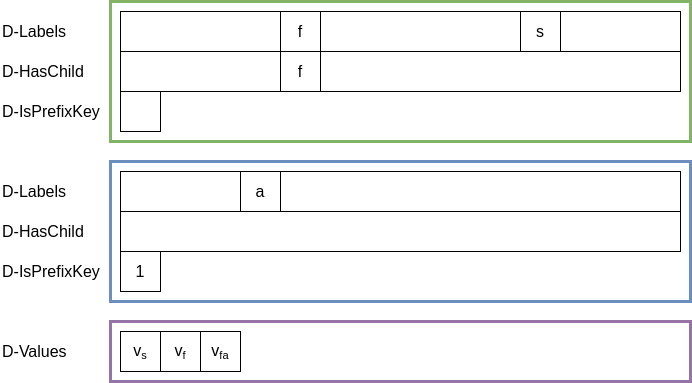
\includegraphics[width=\textwidth]{resources/louds_dense}
						\caption{And its LOUDS-DENSE encoding}
				\end{figure}
		\end{columns}
\end{frame}

\begin{frame}{LOUDS-SPARSE}
\end{frame}

\section{Operations}

\begin{frame}{Building SuRF}
\end{frame}

\begin{frame}{Lookup operations}
\end{frame}

\section{Performance}

\begin{frame}{Performance evaluation}
\end{frame}

\section{Summary \& Q\&A}

\begin{frame}{Summary}
\end{frame}

\section{References}

\begin{frame}[allowframebreaks]
		\frametitle{References}
		\printbibliography
\end{frame}

\end{document}
